\documentclass[12pt]{article}

\usepackage[spanish]{babel}
\usepackage[utf8x]{inputenc}
\usepackage{amsmath}

\usepackage{hyperref}
\usepackage{url}
\usepackage{gensymb}
\usepackage[dvipsnames]{xcolor}

\usepackage{parskip}
\usepackage{fancyhdr}
\usepackage{multicol}
\usepackage{vmargin}
\usepackage{setspace}
\usepackage{geometry}

\usepackage{float}
\usepackage{array}
\usepackage{graphicx}
\graphicspath{{images/}}
\usepackage{wrapfig}
\usepackage{caption}
\usepackage{subcaption}

\setmarginsrb{2 cm}{1 cm}{2 cm}{1.5 cm}{1 cm}{1 cm}{1 cm}{1 cm}

\title{Medición de temperatura}
\author{Martín Alejandro Paredes Sosa}		

\makeatletter
\let\thetitle\@title
\let\theauthor\@author
\let\thedate\@date										
\makeatother

\pagestyle{fancy}
\fancyhf{}
\rhead{Lic.. Física}
\lhead{Informe 3A: \thetitle}
\cfoot{\thepage}

\begin{document}
%%%%%%%%%%%%%%%%%%%%%%%%%%%%%%%%%%%%%%%%%%%%%%%%%%%%%%%%%%%%%%%%%%%%%%%%%%%%%%%%%%%%%%%%
%\begin{titlepage}
%	\centering
%    \vspace*{0.5 cm}
%    
\includegraphics[scale = 0.5]{logo}\\[0.5 cm]	% University Logo
%    \textsc{\LARGE Universidad de Sonora}\\[1 cm]	% University Name
%	\textsc{\Large División de Ciencias Exactas y Naturales}\\[1 cm]		%		% Course Code
%	\textsc{\large Termodinámica Clásica}\\[0.5 cm]				% Course Name
%	\rule{\linewidth}{0.2 mm} \\[0.4 cm]
\begin{center}
{ \large \bfseries \thetitle}\\
\end{center}
%{ \large \bfseries \thetitle}\\
%	\rule{\linewidth}{0.2 mm} \\[1.25 cm]
%    \textsc{\Large Equipo \#2} \\[1.25 cm]
%\thetitle\\	
	\begin{minipage}{\textwidth}
		\begin{center} 
			%\textsc{\Large Integrantes:} \large \\
			\theauthor 
			\end{center}
	\end{minipage}\\[0.2 cm]
%	\vfill
	
%\end{titlepage}
%===================================================================================================
%\pagebreak
%\tableofcontents
%\pagebreak
%===================================================================================================
\begin{abstract}
	Esta practica consistió en realizar mediciones de presión utilizando un termómetro de gas a volumen constante. Mediante la realización que existe entre la presión y la temperatura, se buscó el valor de la temperatura de un recipiente de agua con hielo.
\end{abstract}
\vspace{-1cm}
%===================================================================================================
\section{Introducción}
En está práctica se realizaron mediciones de presión con un \textbf{termómetro de gas a volumen constante (TGVC)} conectado a una interfaz. El objetivo de está práctica es obtener el valor de la temperatura utilizado un TGVC en un recipiente con agua con hielo con la relación que existe entre la presión y temperatura.

Los TGVC se componen de una ampolla con gas (ya se aire, helio, hidrógeno, entre otros) y un manómetro medidor de presión. Utilizando un punto fijo, usualmente se utiliza el punto fijo del agua pero en nuestro caso de se utilizo el punto de fusión normal del agua, podemos obtener la relación entre la temperatura y la presión. En nuestro caso fue la siguiente.

\begin{equation}\label{temlim}
\theta = 273.15 \lim_{P_{sr}\rightarrow 0} \left(\frac{P_{sp}}{P_{sr}} \right)
\end{equation}

%===================================================================================================
\section{Desarrollo Experimental}
En este experimento, primeramente se tenia tres recipiente con agua, dos de ellos se encontraban a temperatura ambiente y el tercero tenia hielo y agua. Luego se tomo nuestro termómetro de gas a volumen constante y en una de sus salidas, se le conecto una bomba de aire, y en otra se conecto un sensor de presión, el cual se encontraba conectado a la interfaz. Este sensor mide en un intervalo de 0 a 700 kPa, con una resolución de 0.5 kPa\cite{man}.

\begin{figure}[H]
\centering
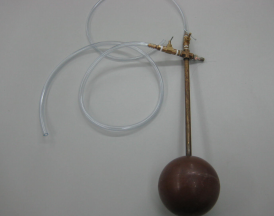
\includegraphics[scale=0.5]{TGVC.png}
\caption{Termómetro de Gas a Volumen Constante}
\end{figure}

\hspace*{0.5cm}Primero se sumergió la ampolla del TGVC en uno de los recipientes con agua a temperatura ambiente. Se espero a que la presión mostrada en la computadora se estabilizara y se tomo el dato. Luego se sumerge en el recipiente con agua y hielo y se espera a que la presión se estabilice para tomar el dato. Luego se sumerge en el tercer recipiente con las misma características que el primero, para no alterar el primer recipiente. Una vez que se estabiliza, con la bomba de aire, se le extrae aire al TGVC para disminuir la presión en su interior, y se sumergió nuevamente en el primer recipiente y se realizo este procedimiento otras 4 veces mas, para así obtener 5 mediciones diferentes.
\begin{figure}[H]
\centering
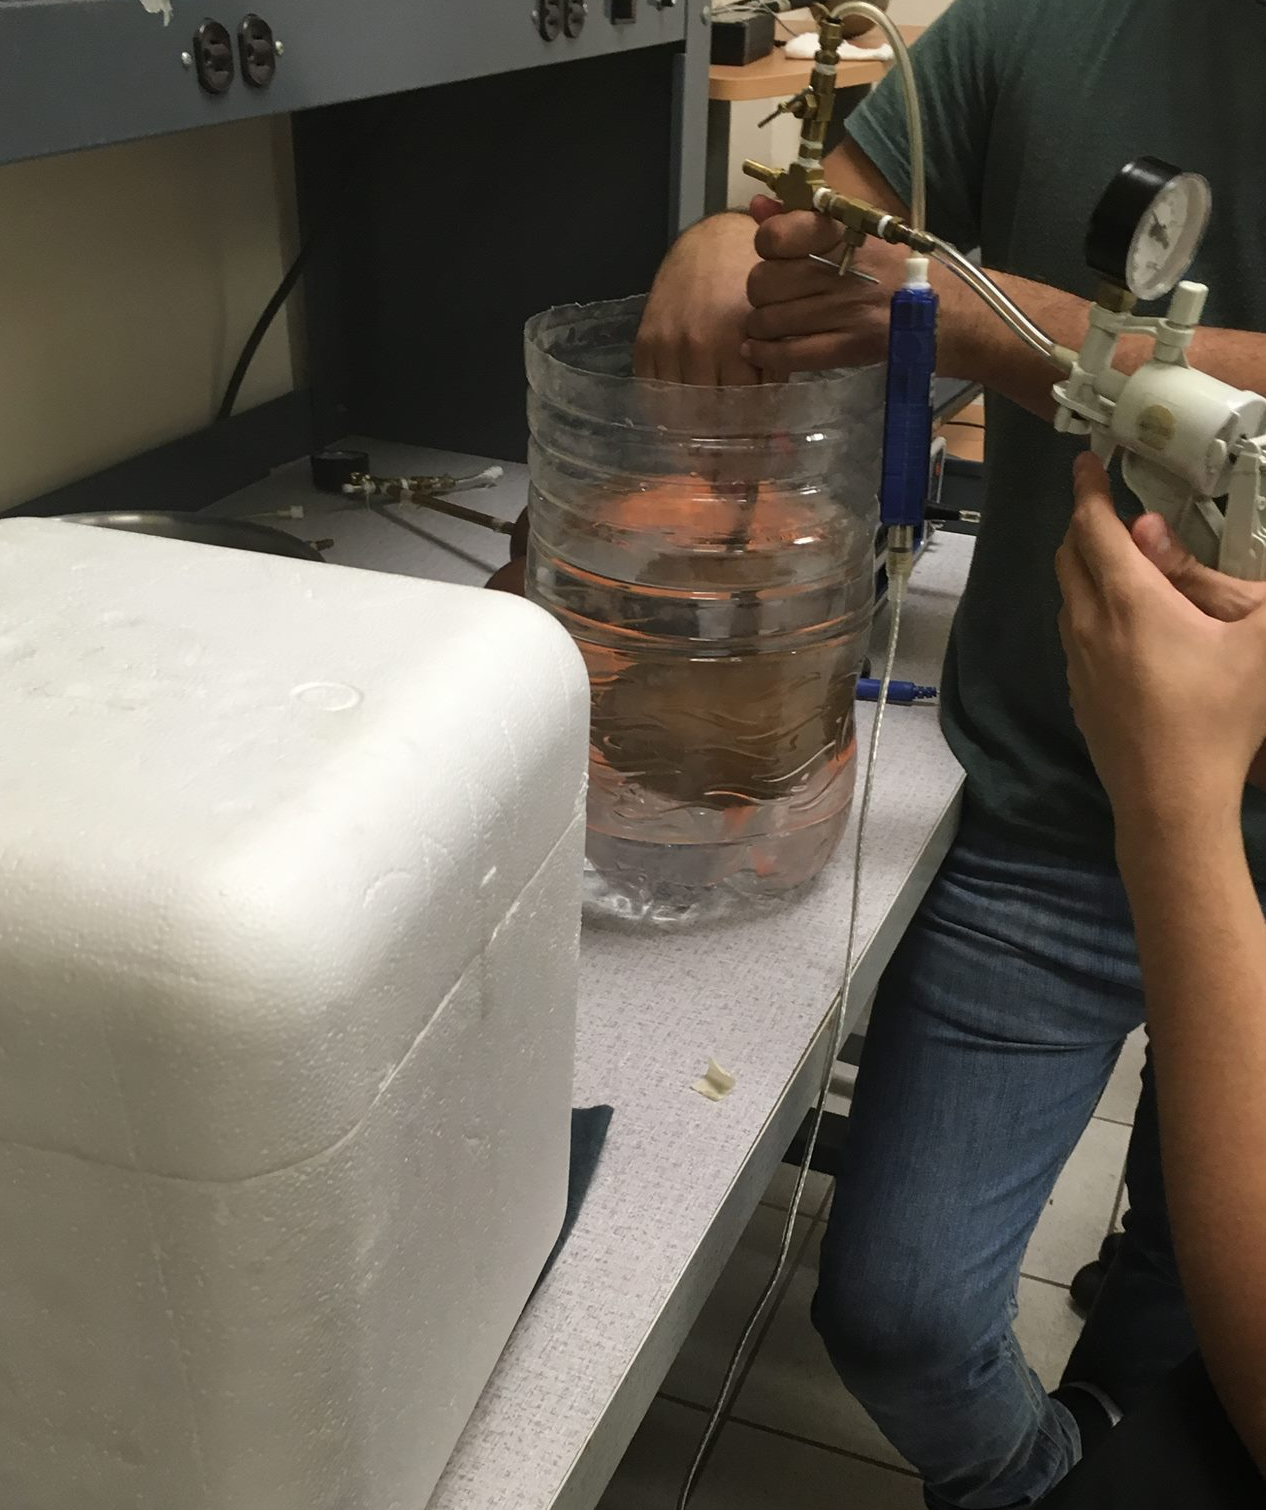
\includegraphics[scale=0.25]{arr.png}
\caption{Arreglo Experimental}
\end{figure}
\pagebreak

%===================================================================================================
\section{Resultados}
Las mediciones que se tomaron de la presión se presentan en la siguiente tabla.

\begin{table}[H]
\centering
\begin{tabular}{|c|c|c|}
\hline
Medición  &  Agua Ambiente(kPa)  &  Agua con hielo(kPa) \\ \hline
   1      &    98.39 $\pm$0.05   &    90.60$\pm$0.05    \\ \hline
   2      &    83.74 $\pm$0.05   &    78.10$\pm$0.05    \\ \hline
   3      &    74.38 $\pm$0.05   &    69.46$\pm$0.05    \\ \hline
   4      &    68.40 $\pm$0.05   &    64.44$\pm$0.05    \\ \hline
   5      &    37.96 $\pm$0.05   &    36.88$\pm$0.05    \\ \hline   
\end{tabular}
\caption{Medición de presiones}
\end{table}
Para poder obtener el valor de la temperatura se hace uso de la ecuación \eqref{temlim}. Esta ecuación nos da la relación que existe entre la temperatura y la presión. En nuestro caso $P_{sp}$ es la presión en el agua ambiente y el $P_{sr}$ es el agua con hielo.
\begin{table}[H]
\centering
\begin{tabular}{|c|c|c|}
\hline
Medición  &  $\dfrac{P_{sp}}{P_{sr}}$ & Temperatura(K)   \\ \hline
   1      &    1.0860     &  296.6361     \\ \hline
   2      &    1.0722     &  292.8756     \\ \hline
   3      &    1.0708     &  293.4978     \\ \hline
   4      &    1.0615     &  289.9358   \\ \hline
   5      &    1.0293     &  281.1490   \\ \hline 
\textbf{Promedio}  & 1.0640  &  290.6188  \\ \hline 
   
\end{tabular}
\caption{Cociente de presiones y Temperatura en Kelvin}
\end{table}

En la siguiente gráfica se muestra la relación entre $P_{sf}$ y el cociente $\dfrac{P_{sp}}{P_{sr}}$

\begin{figure}[H]\label{graph}
\centering
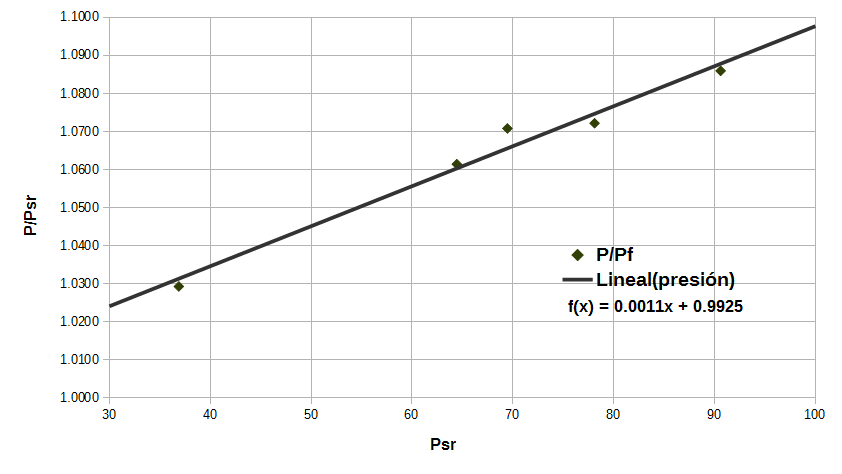
\includegraphics[scale=.55]{grafico.png}
\caption{Relación $P_{sf}$ vs $\frac{P_{sp}}{P_{sr}}$}
\end{figure}

%===================================================================================================
\section{Discusión}
Nuestro experimento nos entregó resultados que se esperaban encontrar. Se noto que al diminuir la presión la temperatura vario mas que cuando se tiene una temperatura ambiente dentro del TGVC. Además se observa que en la gráfica que la relación es lineal.

%===================================================================================================
\section{Conclusiones}
Se puede concluir que en definitiva existe una relación entre la temperatura y la presión cuando el volumen se mantiene constante, gracias al uso del Termómetro de Gas a Volumen Constante. Se observó que con la variación en la presión, se tuvieron valores que se apartaban cada vez mas entre mas se disminuía la presión en el interior del TGVC.

\pagebreak
%================================================================================================


\begin{thebibliography}{6}
	
\bibitem{man}
	\textit{PRESSURE SENSOR - ABSOLUTE}. Recuperado de   \url{http://www.pasco.com}

\bibitem{acu}
Acu\~na, H. (2015). \textit{Manual de Guías de Experiencias en el Laboratorio de Termodinámica Clásica}.

\end{thebibliography}
%================================================================================================

\end{document}

